\chapter{Implementation} \label{chap:Implmentation}

The previous chapter described our proposed \textit{Proactive} flow scheduling algorithm and the design of our experiment. We leverage pre-existing \textit{reactive} flow scheduling decisions in the design of our \textit{Proactive} scheduler. In this chapter, we describe the implementation of our experiment design that has been employed to evaluate the effectiveness of our proposed \textit{Proactive} flow scheduler. In Section \ref{sec:ImplDesc}, an overall description of our design implementation is provided, outlining the working of different major components. In Section \ref{sec:ControlImpl}, the implementations of ECMP, GFF and our \textit{Proactive} flow scheduling SDN controllers are described. Moreover, Section \ref{sec:HadoopEmuImplementation} describes the structure of Hadoop job traces and functional working of the Hadoop emulation. In Section \ref{sec:ThroughputMeasure}, our implementation for measuring throughput from the hosts in the Hadoop emulation is described, and finally, Section \ref{sec:ImplSummary} summarises our design implementation.   


\section{Implementation description} \label{sec:ImplDesc}

We have implemented our \textit{Proactive} flow scheduling algorithm using the \textit{dart} branch \cite{POXdart} of the POX \cite{POXSDN} SDN controller. POX provides an extensible API written in Python, which can be used to program its controlling behaviour. As described in \ref{sec:Emulators}, we use the \textit{Mininet} Network Emulator \cite{lantz2010network} for emulating a 16 host fat-tree data centre topology, where each host is running a Hadoop emulation using \textit{MRemu} \cite{neves2015mremu}. The forwarding behaviour of the switches in the fat-tree network topology is controlled by the POX controller using OpenFlow \cite{mckeown2008openflow}. We run Hadoop jobs and measure Hadoop job completion times along with the total network bandwidth utilization for three flow scheduling algorithms, namely, ECMP \cite{hopps2000analysis}, Global First-Fit \cite{al2010hedera} and our \textit{Proactive} flow scheduling.

Figure \ref{fig:ExecutionOverview} illustrates the working of \textit{LaunchExperiment}, which is the main Python script that initiates the experiment. It builds a \textit{Mininet Network topology object}, by using a script from \textit{Ripl-POX} \cite{riplPOX} to initialize the switch, host and link configurations for a fat-tree network topology. \textit{Ripl-POX} is an extension to the POX controller which provides ECMP hash based routing, as described in \ref{subsec:ECMP}, and Mininet network configurations for data centre topologies such as \textit{fat-tree}, described in \ref{subsec:Fat-Tree Topology}.   

\begin{figure}[!ht] 
	\centerline{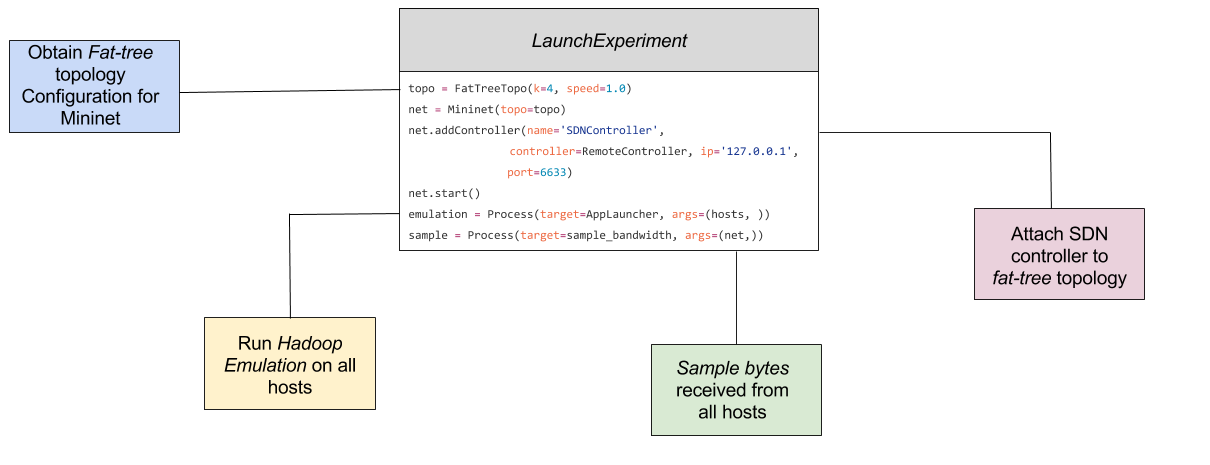
\includegraphics[scale=0.38]{graphics/chapter5/MainExecution.png}}
	\caption{Execution of the main script that loads the different modules of the experiment.}
	\label{fig:ExecutionOverview}
\end{figure}

Subsequently, a remote SDN controller is added to the Mininet network topology object by providing its IP address and port, as illustrated in the Figure \ref{fig:ExecutionOverview}, and the Mininet network emulation is launched. Finally, using Python's Multiprocessing library, two processes are launched simultaneously on each of the 16 hosts, where one of the process runs the Hadoop emulation as described in detail in Section \ref{sec:HadoopEmuImplementation}, while the second process samples the bytes received by the host from its network interface, described in detail in Section \ref{sec:ThroughputMeasure}.

\textit{LaunchExperiment} script illustrated in the Figure \ref{fig:ExecutionOverview} runs the experiment to measure \textit{total bisection bandwidth} achieved and \textit{Hadoop job completion times} when using different SDN remote controllers running on the IP address 127.0.0.1:6633, which are used for evaluating the effectiveness of our \textit{Proactive} flow scheduling against \textit{reactive} scheduling.      


\section{SDN Controller Implementation} \label{sec:ControlImpl}

In this section, we describe the Python-based implementation of our \textit{Proactive} controller along with implementations of ECMP and GFF controllers using the Python API of the POX SDN controller.

\subsection{Equal Cost Multi-Path Routing Implementation} \label{subsec:ECMPImpl}

As mentioned in \ref{sec:ImplDesc}, we used the ECMP routing implementation from \textit{Ripl-POX}, which is an extension of the POX controller.  ECMP routing is described in detail in \ref{subsec:ECMP}. It is the \textit{de-facto} industry standard routing mechanism for multi-path topologies \cite{al2010hedera} described in \ref{sec: DataCentreArch}, and attempts to spread traffic evenly in a network with multiple equal cost paths by hashing selected fields of an incoming packet modulo the total number of paths available and forwarding the packet along the path that corresponds to the result. 

\subsection{Global First-Fit Flow Scheduling Implementation} \label{subsec:GFFImpl}

Global First-Fit flow scheduling is an extension to ECMP routing for scheduling traffic in a topology with multiple equal cost paths between any two source and destination pairs of hosts, described in further detail in \ref{subsec:Hedera}. It maintains link capacities of all paths in the network. When a flow needs to be scheduled, GFF performs a linear search of all possible paths that can accommodate the flow, and allocates the first path that it encounters, which meets the bandwidth demands of the flow.   

The GFF controller class implementation \cite{gffImplementation} used in the experiment is illustrated in Figure \ref{fig:GFFClass}. Once all the switches in the fat-tree topology are connected to the GFF controller, the \textit{\_handle\_ConnectionUp}(event) function stores the switches in a Python list with the switch Data Path IDs which uniquely identify OpenFlow switches, as keys.  

\begin{figure}[!ht] 
	\centerline{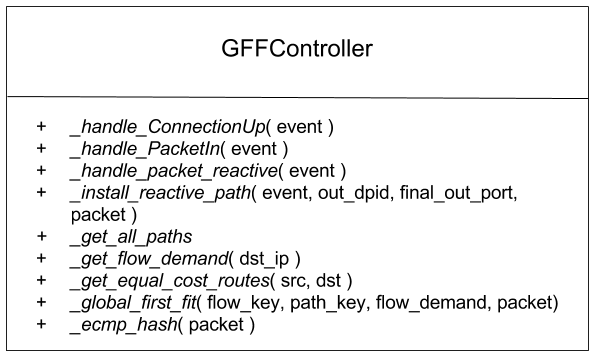
\includegraphics[scale=0.42]{graphics/chapter5/GFFClass.png}}
	\caption{Global First-Fit Network Controller Class}
	\label{fig:GFFClass}
\end{figure}

Subsequently, the \textit{\_get\_all\_paths}() function calculates equal cost routes by calling the \textit{\_get\_equal\_cost\_routes}(src, dst) function for all possible pairs of source and destination nodes in the network. When an OpenFlow switch gets a packet which has no matches in its forwarding table, the packet is sent to the SDN controller for processing \cite{mckeown2008openflow}. This event is handled by the \textit{\_handle\_packet\_reactive}(event) function, which responds by installing a flow entry in the switch, matching the header fields of the packet \textit{reactively}, using the GFF flow scheduling algorithm, and logs the header match fields along with the egress port into a JSON file, to be used later by the \textit{Proactive} controller. 

\subsection{Proactive Controller}

We implemented the \textit{Proactive} Controller on the \textit{hypothesis} that installing flows based on application traffic patterns in a proactive manner will reduce control overhead and high-level latencies caused due to installing of flows \textit{reactively}. Towards this end, we log flow scheduling decisions made by the GFF controller in a JSON file as described in \ref{subsec:GFFImpl}, for a particular Hadoop job. 
\begin{figure}[!ht] 
	\centerline{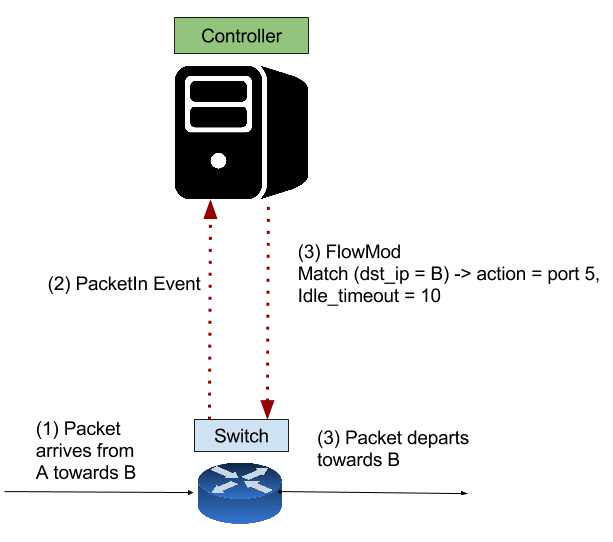
\includegraphics[scale=0.42]{graphics/chapter5/packetinOpenFlow.png}}
	\caption{Handling of \textit{packetIn} event on forwarding table miss by SDN controller using OpenFlow.}
	\label{fig:packetinOpenFlow}
\end{figure}
The same Hadoop job is run again and the logged flows from the previous execution are subsequently fed into the \textit{Proactive} controller, which installs them as soon as all the switches in the network are connected to it. Finally, for every \textit{packetIn} event \textit{i.e.}, when a packet is sent to the controller by a switch since its header fields do not match any entry in the switch's forwarding table as illustrated in Figure \ref{fig:packetinOpenFlow}, the controller procecsses the packet, and based on the control logic running in the controller, it creates \textit{FlowMod} message, with an action specifying the egress port of all packets matching  specific header fields. Subsequently, all packets matching the field as specified in the \textit{FlowMod} message are routed to same egress port by the switch till the entry times out. Similarly, after all the \textit{Proactive} entries time out, the proactive controller behaves like the GFF controller, by routing the packets \textit{reactively} on \textit{packetIn} events. 

Figure \ref{fig:ProactiveClass} illustrates the implementation of the \textit{Proactive} controller class using POX controller's Python API. Similar to the GFF controller class described in \ref{subsec:GFFImpl}, the \textit{\_handle\_ConnectionUp}(event) function stores all switches of the network connected to the controller corresponding to their data path IDs, in a Python list. Additionally, it calls the \textit{\_install\_proactive\_path}() function. 
\begin{figure}[!ht] 
	\centerline{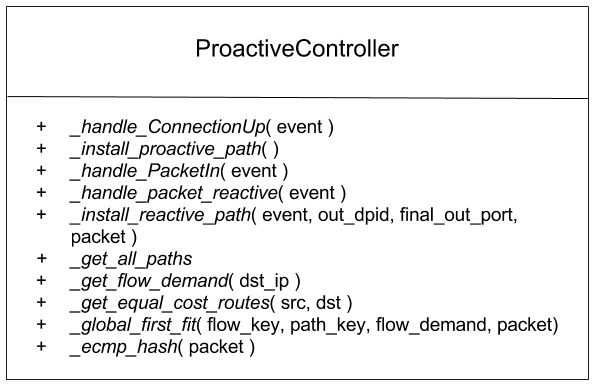
\includegraphics[scale=0.42]{graphics/chapter5/ProactiveClass.png}}
	\caption{Proactive Network Controller Class}
	\label{fig:ProactiveClass}
\end{figure}

The \textit{\_install\_proactive\_path}() function reads all the flow scheduling decisions made by the GFF controller, and installs the same in the appropriate switches. One of the sample flow scheduling decision logged by the GFF controller is illustrated in Figure \ref{fig:FlowRule}.

\begin{figure}[!ht]
\begin{lstlisting}[style=json]
{   
	"dl_type": 2048, 
	"nw_dst": "10.0.0.2", 
	"tp_dst": 6666, 
	"dpid": 1, 
	"tp_src": 48383, 
	"dl_dst": "00:00:00:00:00:02", 
	"dl_vlan": 65535, 
	"nw_src": "10.0.0.3", 
	"dl_src": "00:00:00:00:00:03", 
	"out_port": 2
}
\end{lstlisting}
\caption{Example of a flow decision obtained from GFF flow scheduler which is installed by the \textit{Proactive} network controller.}
\label{fig:FlowRule}
\end{figure}

Notable fields in the log of a flow scheduling decision include \textit{nw\_src}, \textit{nw\_dst}, \textit{dl\_src}, \textit{dl\_dst}, \textit{dpid} and \textit{out\_port} which are the source IP address, destination IP address, source Ethernet address, destination Ethernet address, switch data path ID and the output port respectively. All such logged flow decisions are installed by the \textit{Proactive} controller in the switches along with an \textit{IDLE\_TIMEOUT}, so that switch routing tables are not overwhelmed. Once the flow entries expire, traffic is routed in a \textit{reactive} manner, as described in \ref{subsec:GFFImpl}.   


\section{Hadoop Emulation Implementation} \label{sec:HadoopEmuImplementation}

Since it is not feasible to run a full version of Hadoop on emulated hosts, running on a single machine, due to memory and I/O constraints; therefore, we use a Hadoop emulator MRemu \cite{neves2015mremu}, as discussed in detail in \ref{subsec:Mremu}. It uses traces of real Hadoop Jobs to emulate Hadoop traffic patterns in an emulation running on a single machine, without the need of a real Hadoop cluster. In this section, we describe the structure of Hadoop application traces used in the experiment, and  briefly discuss the functional workflow of the Hadoop emulation.

\subsection{Hadoop Job Traces}

The Hadoop emulator generates traffic patterns in the network on the basis of Hadoop job traces, as discussed in detail in \ref{subsec:Mremu}. The MapReduce applications used to obtain these traces are discussed at length in \ref{sec:BenchTraces}. Information available in the Hadoop job traces is stored in JSON format. Figure \ref{fig:TraceExample} illustrates one element each from the \textit{transfers} and \textit{tasks} JSON arrays in a Hadoop trace. The elements of the \textit{transfer} array provide information about the network transfers and their durations, between two hosts. 

This information is used to generate \textit{iperf} flows between the source and destination hosts for the intended time duration, thereby simulating transfers of the real Hadoop job. 
Similarly, the \textit{task} array provides information pertaining to the different tasks assigned to the hosts in the network and their durations, which are simulated by the corresponding hosts.    

\begin{figure} [!ht]
\begin{lstlisting}[style=json]
{
	"transfers": [{
		"dstAddress": "172.27.102.16",
		"dstPort": 59861,
		"duration": 2.140714136,
		"finishTime": 1388441782.972,
		"mapper": "attempt_201312301708_0016_m_000014_0",
		"reducer": "attempt_201312301708_0016_r_000003_0",
		"size": 62584054,
		"srcAddress": "172.27.102.1",
		"srcPort": 50060,
		"startTime": 1388441780.831286
	}],
	"tasks": [{
		"finishTime": 1388441795.897,
		"host": "172.27.102.1",
		"name": "attempt_201312301708_0016_r_000002_0",
		"processingTime": 6.937,
		"shuffleFinished": 1388441788.953,
		"sortFinished": 1388441788.96,
		"sortingTime": 0.007,
		"startTime": 1388441772.748,
		"type": "REDUCE",
		"waitFinished": 1388441778.417361,
		"waitingTime": 5.669361
	}]
}
\end{lstlisting}
\caption{Example of a Hadoop job trace showing one element each from the transfers
	and tasks JSON arrays.} 
\label{fig:TraceExample}
\end{figure}


\subsection{Functional Architecture}

\textit{LoadExperiment} script executes the Hadoop emulation on all hosts in the network by launching the \textit{AppLauncher} class, as illustrated in Figure \ref{fig:ExecutionOverview}. Functional working of the Hadoop emulation on each host in the network is illustrated in Figure \ref{fig:HadoopEmuArch}. The \textit{AppLauncher} class executes Hadoop emulation on each host by obtaining information about the type of host, \textit{i. e.} if the host is the JobTracker or one of the TaskTrackers from the \textit{TraceParser} class. If the host's IP address corresponds to the JobTracker IP address in the Hadoop trace file, then it assumes the role of the JobTracker \textit{i. e.} the master node in the network, while all other hosts in the network assume the role of TaskTrackers.

\begin{figure}[!ht] 
	\centerline{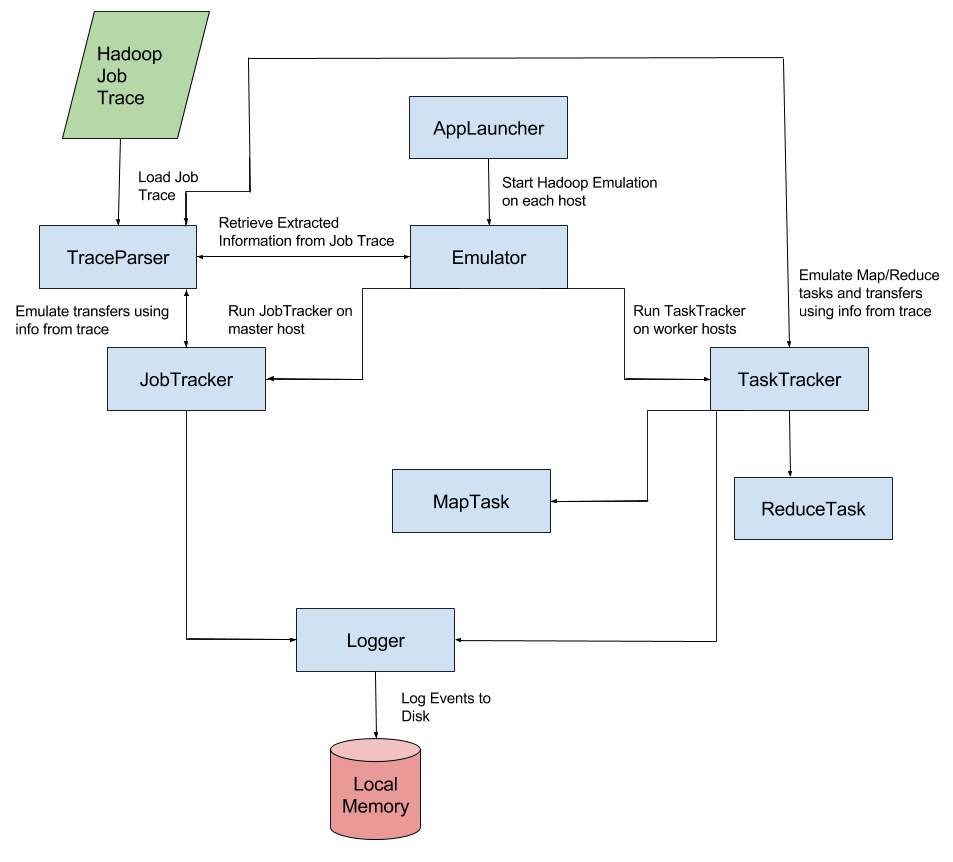
\includegraphics[scale=0.46]{graphics/chapter5/HadoopEmulationArchitecture.png}}
	\caption{Functional Architecture of the Hadoop Emulation.}
	\label{fig:HadoopEmuArch}
\end{figure}

TaskTrackers simulate the working of a Hadoop job by creating \textit{iperf} flows with the same durations as the actual transfer times, which are obtained from the \textit{TraceParser} class. Realistic latencies caused while running \text{Map/Reduce} tasks in Hadoop are also emulated by the TaskTrackers. Similarly, information about  the network traffic generated by the actual JobTracker is used to generate \textit{iperf} flows by the emulated JobTracker. Debug information from the emulated JobTracker and TaskTrackers about network events are logged in disk.      

\section{Throughput Measurement Methodology} \label{sec:ThroughputMeasure}

In this section, the implementation for sampling throughput in the emulated network of our experiment is discussed. In order to measure the total bytes received by a host in the network, we leverage information obtained from \textit{/proc/net/dev} directory of each host in the network.  

The \textit{/proc/} is a virtual Linux filesystem which is made available to user processes by the Linux kernel in order to share internal information about the system \cite{proc}. The \textit{/proc/net/} directory contains a number of files providing some aspect of information on networking of the Linux system. The contents of the files in the \textit{/proc/net/} directory can be viewed by using the \textit{cat} command. One such file in the \textit{/proc/net/} directory is the \textit{/proc/net/dev} file which provides information about the number of bytes transferred and received by the configured network interfaces of the system.      
\begin{figure}[!ht] 
	\centerline{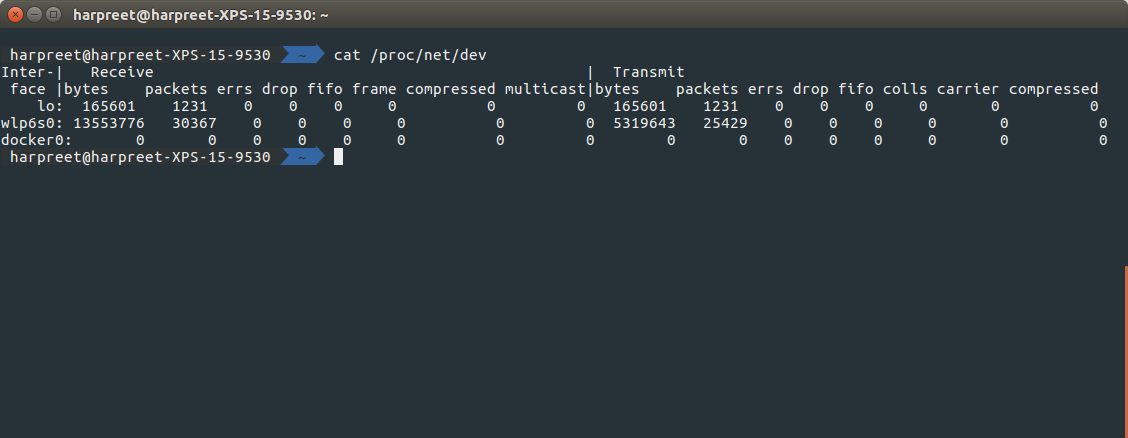
\includegraphics[scale=0.35]{graphics/chapter5/SamplingExample.png}}
	\caption{Sample output of \textit{cat /proc/net/dev} command.}
	\label{fig:ThroughputSamplingEg}
\end{figure}

A sample output of the \textit{cat /proc/net/dev} command is illustrated in Figure \ref{fig:ThroughputSamplingEg}. At any instant, it gives the total number of bytes transmitted and received by the configured network interfaces. This information is leveraged to calculate the total bisection bandwidth achieved by the emulated Hadoop traffic in the network, when routed via \textit{reactive} and \textit{proactive} approaches. 

Once the Hadoop emulation is executed on each host by the \textit{LaunchExperiment} script, it launches the \textit{sample\_bandwidth(net)} function simultaneously, as illustrated in \ref{fig:ExecutionOverview}, which measures the bandwidth used by each host in the network from the \textit{/proc/net/dev} file.

\begin{figure}[!ht] 
	\centerline{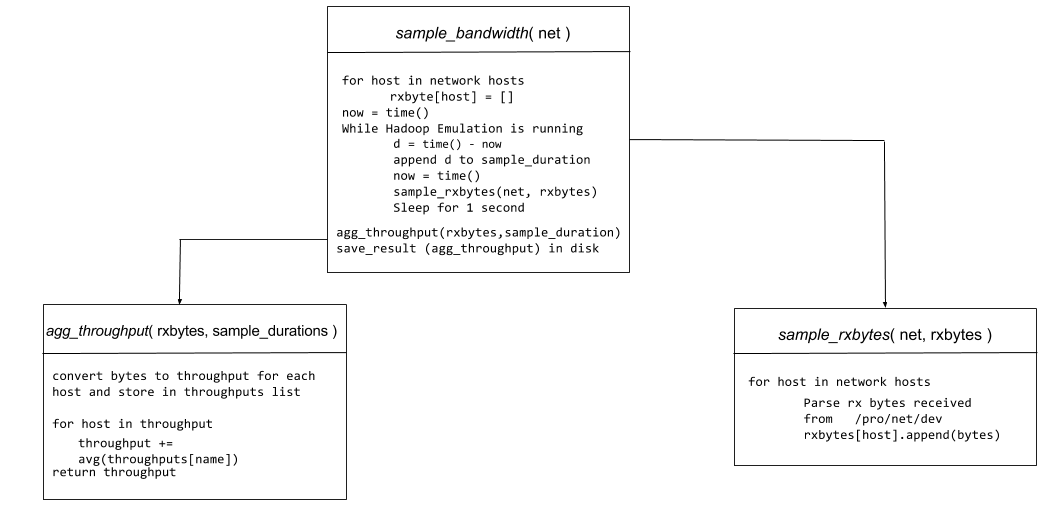
\includegraphics[scale=0.40]{graphics/chapter5/SamplingPseudocode.png}}
	\caption{Pseudocode for sampling of network throughput from all hosts in the network.}
	\label{fig:SamplingPseudocode}
\end{figure}

Pseudocode for sampling bandwidth utilized by each host is illustrated in Figure \ref{fig:SamplingPseudocode}. The \textit{sample\_bandwidth}(net) function creates an empty list of lists with the host objects as keys. Subsequently, while the Hadoop Emulation is running, it captures the total bytes received by the host interface by calling the \textit{sample\_rxbytes}(net, rxbytes) function, and storing the time duration between every two samples in a list. The \textit{sample\_rxbytes}(net, rxbytes) function captures the number of bytes received by the network interface by reading the contents of the \textit{/proc/dev/net} file and stores it in a list corresponding to the host object. 

When the Hadoop emulation terminates, the process of sampling bytes is stopped and the \textit{sample\_bandwidth}(net) function calculates the aggregate throughput achieved by calling the \textit{agg\_throughput}(rxbytes, sample\_durations), where the list of bytes sampled and the the durations of their sampling are sent as parameters. The \textit{agg\_throughput}(rxbytes, sample\_durations) function calculates the total aggregate throughput achieved by all the hosts in the network by converting the bytes to throughputs for each host and subsequently summing the average throughput achieved by each host in the network. 

\section{Summary} \label{sec:ImplSummary}

In summary, we implement the following components based on the design in Chapter \ref{chap:design}
\begin{itemize}
	\item An extension to the Global First-Fit flow scheduling controller which logs its flow scheduling decisions in a JSON file.
	\item A \textit{Proactive} controller that leverages the flow scheduling decisions logged by the Global First-Fit controller, by installing them \textit{proactively} and subsequently defaulting back to the \textit{reactive} behaviour of GFF controller.
	\item A mechanism to sample bytes received by each host in the network via the \textit{/proc/net/dev} directory, which is used to calculate the total throughput achieved by the hosts in the network.   
\end{itemize}


The next chapter discusses the tests carried out to  evaluate our implementation of the \textit{Proactive} flow scheduling mechanism by comparing it against the total throughput achieved by \textit{reactive} routing techniques and the effect of different flow scheduling mechanisms on Hadoop job completion times. 
   